\documentclass[10pt,twoside]{report}
\setlength{\baselineskip}{12pt}
\usepackage{url}
\usepackage{graphicx}
\usepackage{caption}
\usepackage{subcaption}
\usepackage{listings}
\usepackage{xcolor}
\usepackage{framed}
\usepackage{pgfplotstable}
\usepackage{pgfplots}
\usepackage{color}
\lstset{language=Python, keywordstyle=\color{blue}\bfseries, }
\usepackage{amsmath}

\newcommand{\cmnt}[1]{}
%\newcommand{\Transp}[2]{\ensuremath{Tranp(#1,#2)}}
%\newcommand{\Antloc}[2]{\ensuremath{Antloc(#1,#2)}
%\newcommand{\Xcomp}[2]{\ensuremath{Xcomp(#1,#2)}}
%\newcommand{\Eval}[2]{\ensuremath{eval(#1,#2)}}
%\newcommand{\Mod}[2]{\ensuremath{mod(#1,#2)}}

\newcommand{\Alpha}[1]{\ensuremath{\alpha(#1)}}
\newcommand{\Beta}[1]{\ensuremath{\beta(#1)}}
\newcommand{\myGamma}[1]{\ensuremath{\gamma(#1)}}
\newcommand{\myin}[1]{\texttt{In(#1)}}
\newcommand{\myout}[1]{\texttt{Out(#1)}}
\newcommand{\antin}[1]{\texttt{Antin(#1)}}
\newcommand{\antout}[1]{\texttt{Antout(#1)}}
\newcommand{\antloc}[1]{\texttt{Antloc(#1)}}
\newcommand{\transp}[1]{\texttt{Tranp(#1)}}
\newcommand{\xcomp}[1]{\texttt{Xcomp(#1)}}
\newcommand{\availin}[1]{\texttt{Availin(#1)}}
\newcommand{\availout}[1]{\texttt{Availout(#1)}}
\newcommand{\earlin}[1]{\texttt{Earliestin(#1)}}
\newcommand{\earlout}[1]{\texttt{Earliestout(#1)}}
\newcommand{\delayin}[1]{\texttt{Delayin(#1)}}
\newcommand{\delayout}[1]{\texttt{Delayout(#1)}}
\newcommand{\latestin}[1]{\texttt{Latestin(#1)}}
\newcommand{\latestout}[1]{\texttt{Latestout(#1)}}
\newcommand{\isoin}[1]{\texttt{Isolatedin(#1)}}
\newcommand{\isoout}[1]{\texttt{Isolatedout(#1)}}
\newcommand{\insertin}[1]{\texttt{Insertin(#1)}}
\newcommand{\insertout}[1]{\texttt{Insertout(#1)}}
\newcommand{\replacein}[1]{\texttt{Replacein(#1)}}
\newcommand{\replaceout}[1]{\texttt{Replaceout(#1)}}
\pagestyle{myheadings}

\bibliographystyle{siam}

\addtolength{\textwidth}{1.00in}
\addtolength{\textheight}{1.00in}
\addtolength{\evensidemargin}{-1.00in}
\addtolength{\oddsidemargin}{-0.00in}
\addtolength{\topmargin}{-.50in}

\hyphenation{in-de-pen-dent}


\title{\textbf{Partial Redundancy Elimination using Lazy Code Motion}}

\author{Sandeep Dasgupta\thanks{Electronic address:
\texttt{sdasgup3@illinois.edu}} \qquad Tanmay Gangwani\thanks{Electronic
address: \texttt{gangwan2@illinois.edu}}}

\begin{document}
\begin{titlepage}
\thispagestyle{empty}
\maketitle
\pagebreak
\end{titlepage}

\begin{flushleft}
\textbf{\Large{Problem Statement \& Motivation}}
\end{flushleft}
Partial Redundancy Elimination (PRE) is a compiler optimization that eliminates
expressions that are redundant on some but not necessarily all paths through a
program. PRE is a powerful technique since it subsumes Common Subexpression
Elimination (CSE) and Loop Invariant Code Motion (LICM).

In the example below, the computation of the expression (a + b) is partially
redundant because it is redundant on the path $1 \rightarrow 2 \rightarrow 5$,
          but not on the path $1 \rightarrow 4 \rightarrow 5$. PRE works by first introducing
          operations that make the partially redundant expressions fully
          redundant and then deleting the redundant computations. The
          computation of (a + b) is added to 4 and then deleted from 5.


\lstset{ %
  basicstyle=\footnotesize, 
  breakatwhitespace=false,   
  breaklines=true,            
}
\begin{center}
\begin{lstlisting}
    (1) if (OPAQUE)
    (2)   x = a + b;
    (3) else
    (4)   x = 0;
    (5) y=a+b;
\end{lstlisting}
\end{center}

\textcolor{red}{TO DO: Helps in loop invariant code motion}

\begin{flushleft}
\textbf{\Large{Related Work}}
\end{flushleft}
Below we summarize the relevant literature and outline our approach to
implementing a PRE transformation pass in LLVM (\url{http://llvm.org/}).

\begin{description}
\item [Partial Redundancy Elimination]    \hfill \\
Morel et al. \cite{Morel} first proposed a bit-vector algorithm for the
suppression of partial redundancies. The bi-directionality of the algorithm,
            however, proved to be computationally challenging. Knoop et al.
            \cite{Knoop} solved this problem with their Lazy Code Motion (LCM)
  algorithm. It is composed of uni-directional data flow equations and provides
  the earliest and latest placement points for operations that should be
  hoisted. Drechsler et al. \cite{Drechsler} present a variant of LCM which they claim to
  be more useful in practice. Briggs et al. \cite{Briggs2} allude to two
  pre-passes to make PRE more effective - Global Reassociation and Value
  Numbering.

\item [Value Numbering] \hfill \\
Briggs et al. \cite{Briggs} compare and contrast two techniques for
value numbering - hash based\cite{CS} and partition based\cite{AWZ}. In subsequent work they
provide SCC-based Value Numbering \cite{Cooper95scc-basedvalue}  which combines
the best of the previously mentioned approaches. Cooper et al.
\cite{CVDC} show how to incorporate value
information in the data flow equations of LCM to eliminate more redundancies.

\item [LLVM] \hfill \\
Since LLVM is a Static Single Assignment (SSA) based representation, algorithms
based on identifying expressions which are lexically identical or have the same
static value number may fail to capture some redundancies.
%as shown in figure
%below. <slide 5 picture in Karkare>. 
Keneddy Chow et al.
\cite{Kennedy99partialredundancy} provide a new framework for PRE on a program
in SSA form. The present GVN-PRE pass in LLVM appears to be inspired by the
work of Thomas et al. \cite{Vandrunen04value-basedpartial} which also focusses
on SSA.
\end{description}

\begin{flushleft}
\textbf{\Large{Our Aproach}}
\end{flushleft}

\begin{itemize}
\item  In this project, we implemented the iterative bit-vector
data flow algorithm inspired by LCM \cite{Knoop}. It uses five data flow equations to
identify optimal placement points for hoisting. The first two - anticipatable
and earliest - calculate the computationally optimal placement and the next
three - latest (in 2 steps) and isolated - calculate the lifetime optimal
placement.  The final step of the algorithm entails inserting new code and
removing redundant expressions. All critical edges\footnote{Edges from blocks
  with more than one successor to blocks with more than one predecessor } are
  removed prior to starting LCM.

\item As suggested in \cite{Briggs2}, running two pre-passes produces code more
amenable to PRE. We plan to use an already existing LLVM pass (-reassociate)
  for Global Reassociation.  We have implemented our own pass for Value Numbering
  using the approach outlined in \cite{Cooper95scc-basedvalue}. This is based
  on Tarjan's SCC algorithm. It works on the strongly connected components of
  the SSA graph as opposed to the CFG. The algorithm combines the ability to
  perform constant folding and algebraic simplifications with the ability to
  make optimistic assumptions (and later disprove them). Because of this, it
  can find at least as many equivalences as the hashing or partitioning based
  approach.

\item To incorporate information from the Value Numbering pass into the LCM pass,
  we modified the flow equations to work on \emph{values} rather than
  lexical names. \cite{CVDC} details how the flow equations
  change for a variant of LCM. We make the observation that only ANTLOC and
  TRANSP predicates would need to be suitably modified to handle \emph{values}.
\end{itemize}

The following is the detailed explanation od our approach.

\begin{flushleft}
\textbf{\large{Value Numbering}}
\end{flushleft}

Prior research has shown that value numbering can increase opportunities for PRE.
LLVM presently has a GVN-PRE pass which exploits this. However, value numbering in 
GVN-PRE is tightly coupled with the code for removing redundancies, and hence
we deem it not useful for our purposes. We have written our own value numbering
pass which feeds expression value numbers to the PRE stage. It should be noted,
     however, that we do not implement value numbering from scratch and use an
     old (now defunct) LLVM pass as a starting point. Most importantly, we
     augment the basic value numbering in the following ways - 
     
\begin{itemize}     
  \item Add the notion of leader expression (described below), with associated
  data structures and functions. 
  \item Functionality to support value-number-based bitvectors rather than
  expression-name-based bitvectors. 
  \item (Optimization 1) If the expression operator is one of these - AND, OR, CMP::EQ
  or CMP::NE, and the operands have the same value number, we replace all uses
  accordingly and then delete the expression.
  \item (Optimization 2) If all operands of an expression are constants, then we 
  evaluate and propagate constants. 
  \item (Optimization 3) If one operand of an expression is a constant (0 or 1), then 
  we simplify the expression. e.g. {a+0 = a} , {b*1 = b}.
  \item (Optimization 4) If the incoming expressions to a \texttt{Phi} node have the same value 
  number, then the \texttt{Phi} node gets that same value number
\end{itemize}  
  As per our testing, optimizations 2 and 3 are also done by the reassociation
  pass in LLVM. In our final code we omit our implementation and rely on the
  more robust LLMV pass. Optimizations 1 and 4, however, are still our contribution.

\begin{flushleft}
\textbf{\large{Notion Of Leader Expression}}
\end{flushleft}
The value numbering algorithm computes the RPO solution as outlined in
\cite{Cooper95scc-basedvalue}. It goes over the basic blocks in reverse post
order and adds new expressions to a hash table based on the already computed
value numbers of the operands. We call an expression a `leader' if at the time
of computing its value number, the value number doesn't already exist in the
hash table. In other words, out of a potentially large set of expressions that
map to a particular value number, the leader expression was the first to be
encountered while traversing the function in reverse post order. Leader
expressions are vital to our algorithm as they are used to calculate the block
local properties of the dataflow equations.

\begin{flushleft}
\textbf{\large{Types Of Redundancies}}
\end{flushleft}
Given two expression X and Y in the source code, following are the possibilities - \\
\indent1. X and Y are lexically equivalent, and have the same value numbers \\
\indent2. X and Y are lexically equivalent, but have different value numbers \\
\indent3. X and Y are lexically different, but have the same value numbers \\
\indent4. X and Y are lexically different, and have different value numbers \\
In the source code, there could be opportunities for redundancy elimination in
cases 1, 2 and 3 above. If the source code is converted to an intermediate
representation in SSA form then case 2 becomes an impossibility (by guarantees of SSA). Therefore,
               our algorithm presently handles the cases when X and Y are
               lexically same/different, but both have the same value number (cases 1 and 3).
               Driven by this observation, we implement value number based code
               motion, the details of which are presented below. It should be
               noted that even though case 2 above is not possible in SSA,
               the source code redundancies  of this type transform into that
               of type case 4. Figure \ref{fig:0} presents an illustration of the same. \textbf{This is not handled
               in the current implementation.} 
\begin{figure}[htbp]
  \begin{center}
    \scalebox{.6}{\begin{tabular}{@{}p{12cm}@{ } @{ }p{12cm}@{}}
     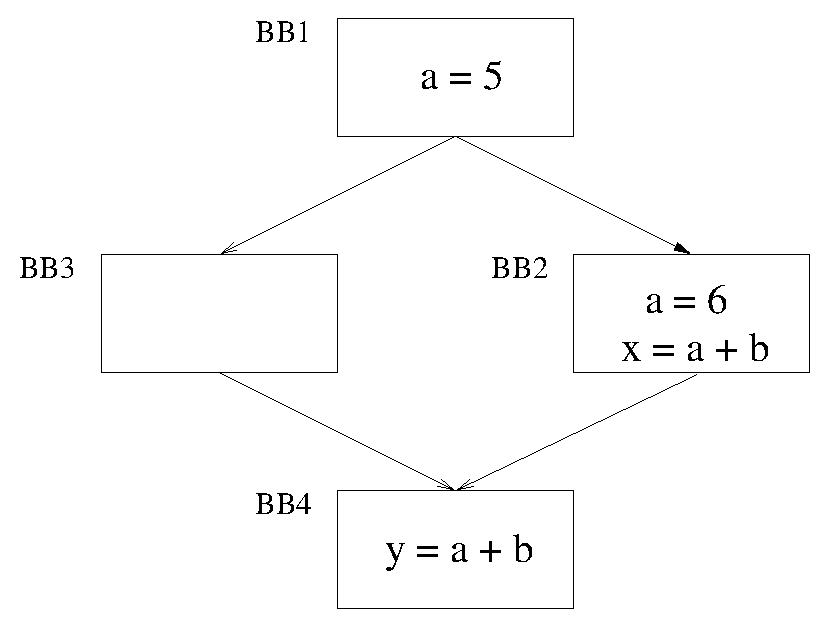
\includegraphics[scale=0.8]{Figs/3} & 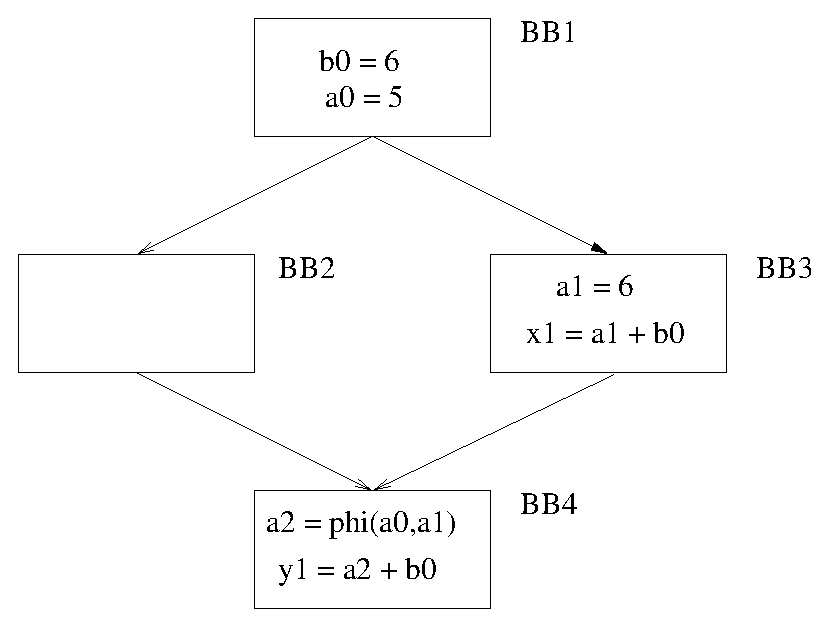
\includegraphics[scale=0.8]{Figs/4} \\
      &\\
  \text{Code not in SSA Form; Two lexically equivalent expressions} &
  \text{Code in SSA Form; Two lexically different expressions} \\
  \text{in Basic block 3 and 4 with different value numbers.} &
  \text{in Basic block 3 and 4 with different value numbers.}
    \end{tabular}}
  \end{center}
  \caption{\label{fig:0} }
\end{figure}

\begin{flushleft}
\textbf{\large{Value-Number driven code motion}}
\end{flushleft}
We implement an iterative bit vector data flow algorithm for PRE. We initially
implemented the flow equations from the Lazy Code Motion paper. This set
included a total of 13 bit vectors for each basic block - 2 for block local
properties ANTLOC and TRANSP, and 11 for global properties. These equations,
           however, could only be applied to single instruction basic blocks.
           We therefore, derived a new set of equations which are motived by
           later work\cite{Knoop:1994:OCM:183432.183443} of the same authors.
           This set of equations apply to maximal basic blocks and
           entails a total of 19 bit vectors for each basic block in our
           current implementation - 3 for block local properties ANTLOC,
           TRANSP, XCOMP and 16 for global properties.  We include the
           data flow framework, and show how each PRE equation maps to the
           framework. We call the algorithm value-number driven because each
           slot in each of the bit vectors is reserved for a particular value
           number rather than a particular expression. Also, we make the
           observation that a large number of expressions in the program only
           occur once, and are not useful for PRE. Hence to further optimize
           for space and time, we only give bit vector slots to value numbers
           which have more than one expression linked to them.

\begin{flushleft}
\textbf{\large{Local CSE}}
\end{flushleft}
For our data flow equations to work correctly, a local CSE pass has to be run
on each basic block. Basically, this path removes the redundancies inside
straight line basic block code and sanitizes it for the iterative bit vector
algorithm. This idea is borrowed from \cite{Knoop:1994:OCM:183432.183443}. We perform this step before calling
our data flow framework. 
\textcolor{red}{TO DO: Why needed.}

\begin{flushleft}
\textbf{\large{Insert and Replace}}
\end{flushleft}
To maintain compatibility with SSA, we perform insertion and replacement
  through memory and re-run the \emph{mem2reg} pass after our PRE pass to convert the
  newly created load and store instructions to register operations. Following
  are the major points:
\begin{itemize}  
  \item Assign stack space \emph{(allocas)} at the beginning of the
  function for all the expressions that need movement
  \item At insertion point,
           compute the expression and save the value to the stack slot assigned to the
             expression 
  \item At replacement point, load from the correct stack
             slot, replace all uses of the original expression with the load
             instruction, and delete the original expression
  \item \emph{mem2reg} converts stack operations to register operations and introduces the 
             necessary ${\Phi}$ instructions
\end{itemize}  

In appendix D, we have shown that in Figure\ref{fig:1}
and Figure\ref{fig:2}, the optimizations performed by our PRE pass. The intention here is to
  show how our version of PRE performed on the computations $a + b$ \& $a < b$;

One point about the insertion step is worth mentioning. Suppose that an
expression, with value number vn, is to be inserted in a basic block.
Although our algorithm can handle all cases, for simplicity, assume that the
insertion point is the end of the basic block. To insert the expression we
scan the list of the expressions in the whole function which have the same
value number vn.  We then clone one of these expressions (called provider)
  and place at the end of the basic block. The trivial case is when the the
  provider is available in the same basic block. If however, the provider
  comes from another basic block, then we need to ensure that the operands
  of the provider dominate the basic block where we wish to insert the
  expression in. Not being able to find a suitable provider is the only case
  where we override the suggestion of the data flow analysis and not do PRE
  for that expression only. PRE for other expressions proceeds as usual. Our
  initial testing suggests that this is a very rare occurrence. 

\begin{flushleft}
\textbf{\Large{Loop Invariant Code Motion}}
\end{flushleft}
We first address a question raised in the phase-1 report. We had previously
mentioned that to optimize for space and time, we provide a bit vector slot only to
value numbers which have more than one expression linked to them. With this,
      however, we could miss opportunities for loop invariant code motion. As a
      solution, we extend the bit vector to include value numbers which have
      only a single expression linked to them but only if the expression is
      inside a loop. Note that we still exclude the cases where the expression
      is not part of a loop, and expect reasonable space and time savings.  

      The second issue we resolved with respect to loop invariant code motion was 
      checking for zero-trip loops. Our PRE algorithm would move the loop invariant
      computations to the loop pre-header only if placement in the loop pre-header is 
      anticipatible. Such a pre-header is always available for \emph{do-while} loops, 
      but not for \emph{while} and \emph{for} loops. Hence, a modification is required
      to the structure of \emph{while} and \emph{for} loops which peels off the first
      iteration of the loop, protected by the loop condition. This alteration provides 
      PRE with a suitable loop pre-header to hoist loop independent computations to.
      In Figure \ref{fig:5} we show the CFG changes. Fortunately, we were able to 
      achieve this effect using an existing LLVM pass \emph{-loop-rotate} rather than
      having to write it ourselves.

\begin{figure}[htbp]
  \begin{center}
     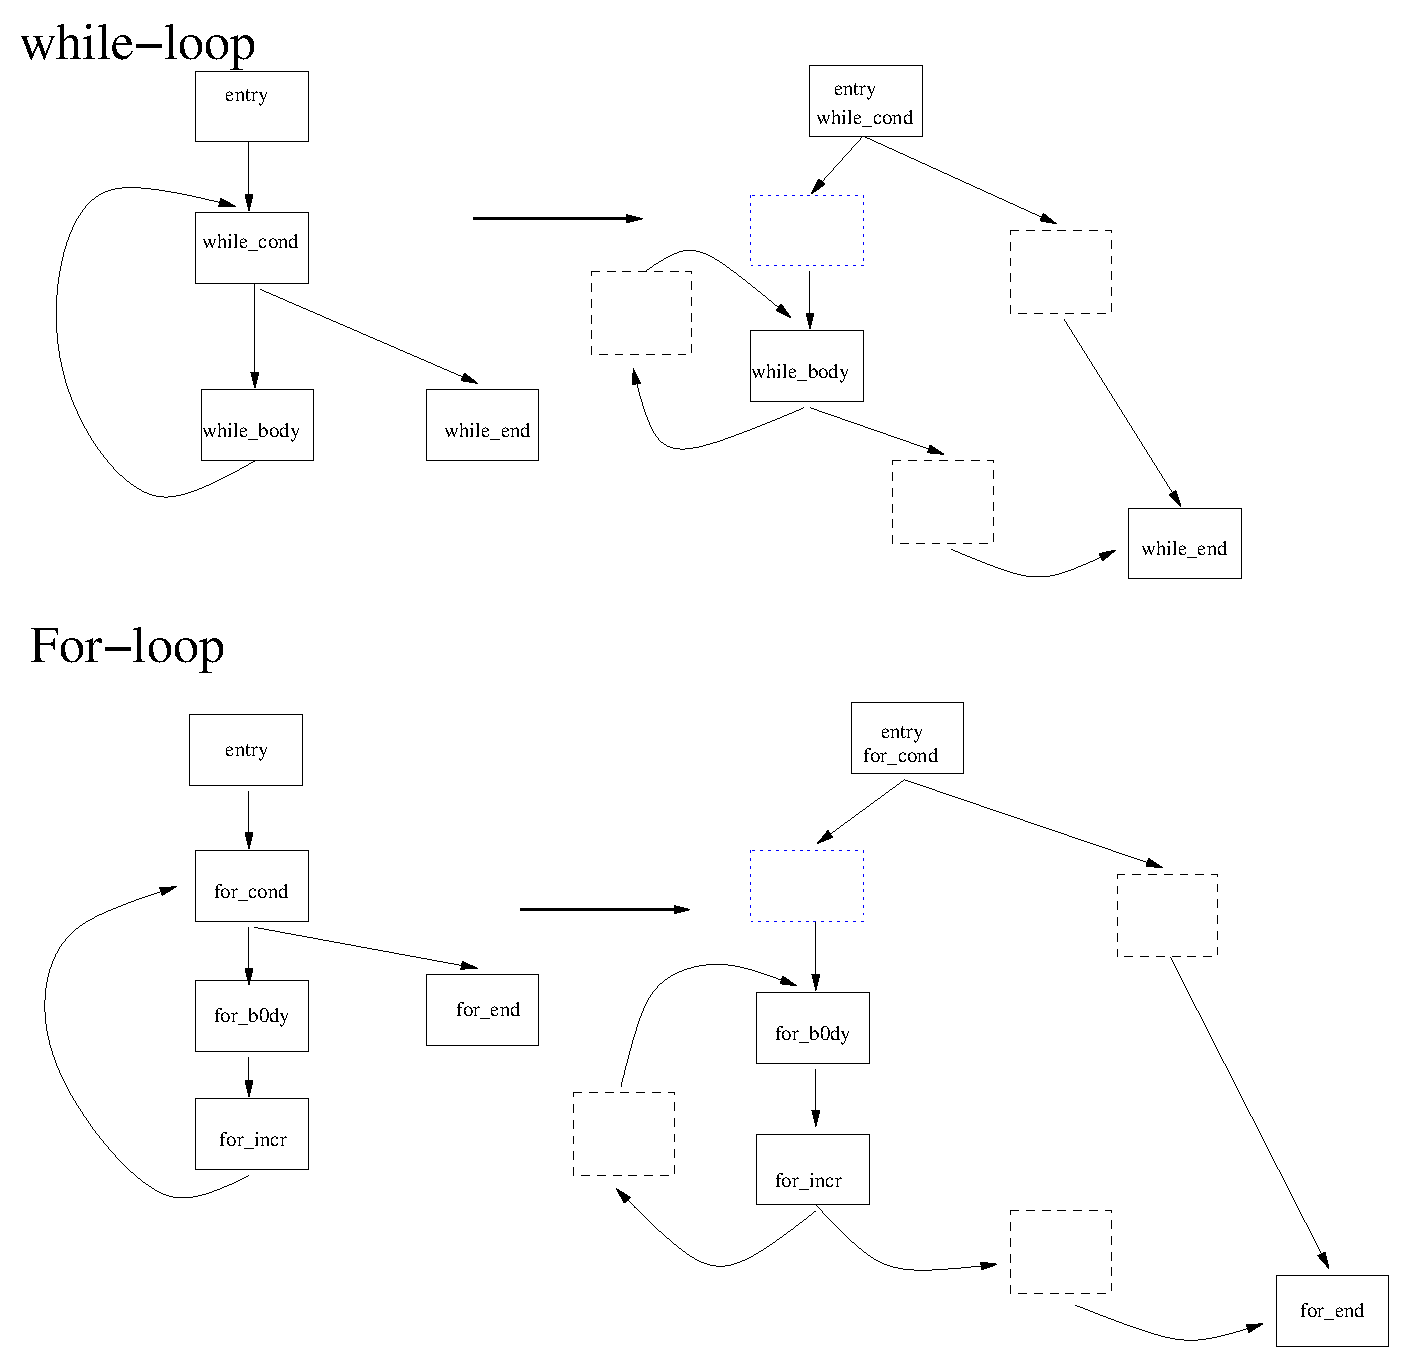
\includegraphics[scale=0.5]{Figs/5} 
  \end{center}
  \caption{Loop transformations done by \emph{-loop-rotate}. \emph{do-while}
    loops remain unaffected. Blue dotted boxes are the ones inserted by loop
      rotate. PRE can insert the computations in these places.}
  \label{fig:5} 
  \end{figure}


\newpage  
\begin{flushleft}
\textbf{\Large{Testing}}
\end{flushleft}

Apart from the small test cases which we created in phase-1, we have been able to 
successfully test our PRE pass on real codes from the LLVM test-suite. Specifically, we have
completed the testing for 75 benchmarks from LLVM single-source package \emph{"test-suite/SingleSource/Benchmarks/"} for correctness and performance. Correctness is checked by
comparing the output of the binary optimized with our PRE pass with the reference output 
provided along with benchmarks. All benchmarks pass the correctness test. For performance, 
we compile the codes with and without the PRE pass and take the ratio of the run-times on 
the hardware. Figure 4 shows the S-curve for performance. For 55/75 benchmarks, our pass improves 
the run time by varying amounts (upto 67\%). Performance drops for few benchmarks, but the degradation is bound by 8\%.

Apart from measured runtime on the hardware, another metric to quantify the
effects of our optimization pass is the dynamic instruction count. We use Pin
(dynamic binary instrumentation tool) from Intel for this purpose. We have
written a very simple Pintool to dump the dynamic instruction count of each
type of instruction. We would present supporting data from Pin our final
report.
%\pgfplotstabletypeset{Data/data.dat}

\begin{figure}
\begin{center}
\begin{tikzpicture}
\begin{axis}[
  xlabel=Benchmark number,
  ylabel=Base Time/ PRE Time,
  ymax=1.7, ymin=0.8, xmax=80,
  x tick label style={black},
  grid=both,xmajorgrids=false,
  ]
\addplot table [y=T, x=N]{Data/data.dat};
\end{axis}
\end{tikzpicture}
\end{center}
\label{fig:6}
\caption{S-curve for performance improvements over Baseline (no PRE)}
\end{figure}

\begin{flushleft}
\textbf{\Large{{Conclustion and Future Work }}}
\end{flushleft} 
In this phase, we were able to code the missing pieces of our PRE algorithm,
   thereby achieving full functionality of the project. The highlights were the
   insert-replace algorithm, LICM improvements, and fixes for numerous bugs
   which surfaced during testing on the LLVM single-source package. We have
   written scripts to automate the testing, and this would speed up work for
   the final phase. \\ 
   The S-curve in this report (Figure 5)
   presents improvements with respect to the baseline (no PRE pass) for
   single-source package. We would like to evaluate the cases where our pass
   degrades performance compared to baseline. In our final report, we plan to
   include similar curves for benchamarks from the LLVM multi-source package as
   well as the SPEC 2006 suite. Also, we would include S-curves to compare the
   effectiveness of our PRE pass with the LLVM GVN-PRE pass. For extreme
   outliers, we hope to present supporting data to reason about the performance
   change. Pin tool analysis and the statistics dumped by our PRE pass would be
   used for this.

\appendix

\chapter{Computation of localized sets}
For each basic block there are 3 bit vectors dedicated to the block-specific
properties, namely \texttt{Transp}, \texttt{Antloc} and \texttt{Xcomp}. As mentioned before, a bit vector
is a boolean array of value numbers. Each value number is associated with
at-least two expressions from the IR. Let the leader
expression (as defined in the section on value numbering) associated with the
value number $v$ be called $L(v)$. 


\begin{equation}
\begin{array}{l c l}
\texttt{Transp(v,B)} &=& \left\{
                    \begin{array}{l l}
                        false & \quad \text{iff $\exists$ x $\in$ operands of L(v) such that \texttt{Mod(x,B)} = true}\\
                        true & \quad \text{Otherwise}
                    \end{array} \right. \\
\texttt{Antloc(v,B)} &=& \texttt{Eval(v,B)} \cap \texttt{Transp(v,B)} \\
\texttt{Xcomp(v,B)} &=& \texttt{Eval(v,B)} \cap \overline{\texttt{Transp(v,B)}}\\
  &&\\
\text{where}&& \\  
\quad \texttt{Eval(v,B)} &=& \text{\{v $|$ value number v is computed in B\}}\\
\quad \texttt{Mod(op,B)} &=& \text{operand op modified in B}\\
\end{array}
\end{equation}

\chapter{Lazy Code motion Transformations}

\begin{itemize}
\item Down Safety Analysis (Backward data flow analysis)
\begin{equation}
\begin{array}{l c l}
\antin{b} &=& \antloc{b} \cup (\transp{b} \cap \antout{b}) \\
\antout{b} &=& \xcomp{b} \cup \left\{
                    \begin{array}{l l}
                        \phi & \quad \text{if b = exit}\\
                        \displaystyle \bigcap_{s \in succ(b)} \antin{s} &
                    \end{array} \right. \\
\end{array}
\end{equation}

\item Up Safety Analysis (Forward data flow analysis)
\begin{equation}
\begin{array}{l c l}
\availin{b} &=& \left\{
                  \begin{array}{l l}
                        \phi & \quad \text{if b = entry}\\
                        \displaystyle \bigcap_{p \in pred(b)} (\xcomp{p} \cup \availout{p}) & 
                  \end{array} 
              \right. \\
\availout{b} &=& \transp{b} \cap (\antloc{b} \cup \availin{b}) \\
\end{array}
\end{equation}

\item Earliest-ness (No data flow analysis)
\begin{equation}
\begin{array}{l c l}
\earlin{b}  &=& \antin{b} \cap \displaystyle \bigcap_{p \in pred(b)} (\overline{\availout{p} \cup \antout{p}}) \\ 
\earlout{b} &=& \antout{b} \cap \overline{\transp{b}}
\end{array}
\end{equation}

\item Delayability (Forward data flow analysis)
\begin{equation}
\begin{array}{l c l}
\delayin{b} &=& \earlin{b} \cup  \left\{
                              \begin{array}{l l}
                                \phi & \quad \text{if b = entry}\\
                                \displaystyle \bigcap_{p \in pred(b)} (\overline{\xcomp{p}} \cap \delayout{p}) & 
                  \end{array} 
              \right. \\
\delayout{b} &=& \earlout{b} \cup (\delayin{b} \cap \overline{\antloc{b}}) \\
\end{array}
\end{equation}

\item Latest-ness (No data flow analysis)
\begin{equation}
\begin{array}{l c l}
\latestin{b}  &=& \delayin{b} \cap \antloc{b}\\
\latestout{b} &=& \delayout{b} \cap (\xcomp{b} \cup \displaystyle \bigcup_{s \in succ(b)} \overline{\delayin{s}})
\end{array}
\end{equation}


\item Isolation Analysis (Backward data flow analysis)
\begin{equation}
\begin{array}{l c l}
\isoin{b} &=& \earlout{b} \cup \isoout{b} \\
\isoout{b} &=& \left\{
                    \begin{array}{l l}
                        U & \quad \text{if b = exit}\\
                        \displaystyle \bigcap_{s \in succ(b)} (\earlin{s} \cup (\overline{\antloc{s}} \cap \isoin{s}) )&
                    \end{array} \right. \\
\end{array}
\end{equation}

\item Insert and Replace points
\begin{equation}
\begin{array}{l c l}
\insertin{b} &=& \latestin{b} \cap \overline{\isoin{b}} \\
\insertout{b} &=& \latestout{b} \cap \overline{\isoout{b}} \\
&&\\
\replacein{b} &=& \antloc{b} \cap \overline{\latestin{b} \cap \isoin{b}} \\
\replaceout{b} &=& \xcomp{b} \cap \overline{\latestout{b} \cap \isoout{b}}
\end{array}
\end{equation}
\end{itemize}

\chapter{Generalized data flow framework}

All the equations in Appendix B can be computed using the generic
framework defined below.

\section{Forward Analysis}
\begin{equation}
\begin{array}{l c l}
\myin{b} &=& \Alpha{b} \cup  \left\{
                    \begin{array}{l l}
                        \bot & \quad \text{if b = entry}\\
                        \displaystyle \bigwedge_{p \in pred(b)} \Beta{p}&
                    \end{array} \right. \\
\myout{b} &=& \myGamma{b}                      
\end{array}
\end{equation}

\section{Backward Analysis}
\begin{equation}
\begin{array}{l c l}
\myin{b} &=& \myGamma{b}                      \\
\myout{b} &=& \Alpha{b} \cup  \left\{
                    \begin{array}{l l}
                        \bot & \quad \text{if b = exit}\\
                        \displaystyle \bigwedge_{s \in succ(b)} \Beta{s}&
                    \end{array} \right. \\
\end{array}
\end{equation}

The following is the function which we call with dataflow equation
specific parameters defined subsequently.

\begin{framed}
\[
\texttt{callFramework}(\myout{b}, \myin{b}, \Alpha{b}, \Beta{b},\myGamma{b}, \bigwedge, \bot, \top, \text{Direction})
\]
\end{framed}

Following is the list of values that we need to plug-in to $\alpha$,
          $\beta$ and $\gamma$ for the above generic framework
          to work.



\begin{itemize}
\item Down Safety Analysis (Backward data flow analysis)
\begin{equation}
\begin{array}{l c l}
\Alpha{x}     &=& \xcomp{x} \\
\Beta{x}      &=& \antin{x}     \\     
\myGamma{x}   &=& \transp{x} \cap \antout{x} \cup \antloc{x}\\
\bigwedge     &=&  \cap \\
\bot          &=& \phi \\
\top          &=& V, \text{set of all values} \\
\text{Direction}    &=& \text{Backward}
\end{array}
\end{equation}

\item Up Safety Analysis (Forward data flow analysis)
\begin{equation}
\begin{array}{l c l}
\Beta{x}      &=& \xcomp{x} \cup \availout{x}     \\     
\myGamma{x}   &=& \antloc{x} \cup \availin{x} \cap \transp{x}\\
\bigwedge     &=&  \cap \\
\bot          &=& \phi \\
\top          &=& V, \text{set of all values} \\
\text{Direction}    &=& \text{Forward}
\end{array}
\end{equation}

\item Delayability (Forward data flow analysis)
\begin{equation}
\begin{array}{l c l}
\Alpha{x}     &=& \earlin{x} \\
\Beta{x}      &=& \overline{\xcomp{x}} \cap \delayout{x}     \\     
\myGamma{x}   &=& \delayin{x} \cap \overline{\antloc{x}} \cup \earlout{x}\\
\bigwedge     &=&  \cap \\
\bot          &=& \phi \\
\top          &=& V, \text{set of all values} \\
\text{Direction}    &=& \text{Forward}
\end{array}
\end{equation}

\item Isolation Analysis (Backward data flow analysis)
\begin{equation}
\begin{array}{l c l}
\Beta{x}      &=& \overline{\antloc{x}} \cap \isoin{x} \cup \earlin{x}     \\     
\myGamma{x}   &=& \earlout{x} \cup \isoout{x} \\
\bigwedge     &=&  \cap \\
\bot          &=& V, \text{set of all values} \\
\top          &=& V, \text{set of all values} \\
\text{Direction}    &=& \text{Backward}
\end{array}
\end{equation}

\end{itemize}

   
\nocite{*}
\bibliography{report}
  
\end{document}
